\chapter{Intersection Algorithms\label{intersect}}

In this chapter we are going to see a collection of algorithms to compute the intersection of two \textbf{sorted} lists, taken from the chapter six of "Pearl of Algorithm Engineering" by Paolo Ferragina, published by Cambridge University Press \citep{Ferragina_2023}. \\
We will first look at two of the most commonly used search algorithms, since we cannot intersect without searching. \\

\section{Search Algorithms}

\subsection{Binary Search \label{sec:binsearch}}

\begin{figure}[ht] 
    \begin{center}
        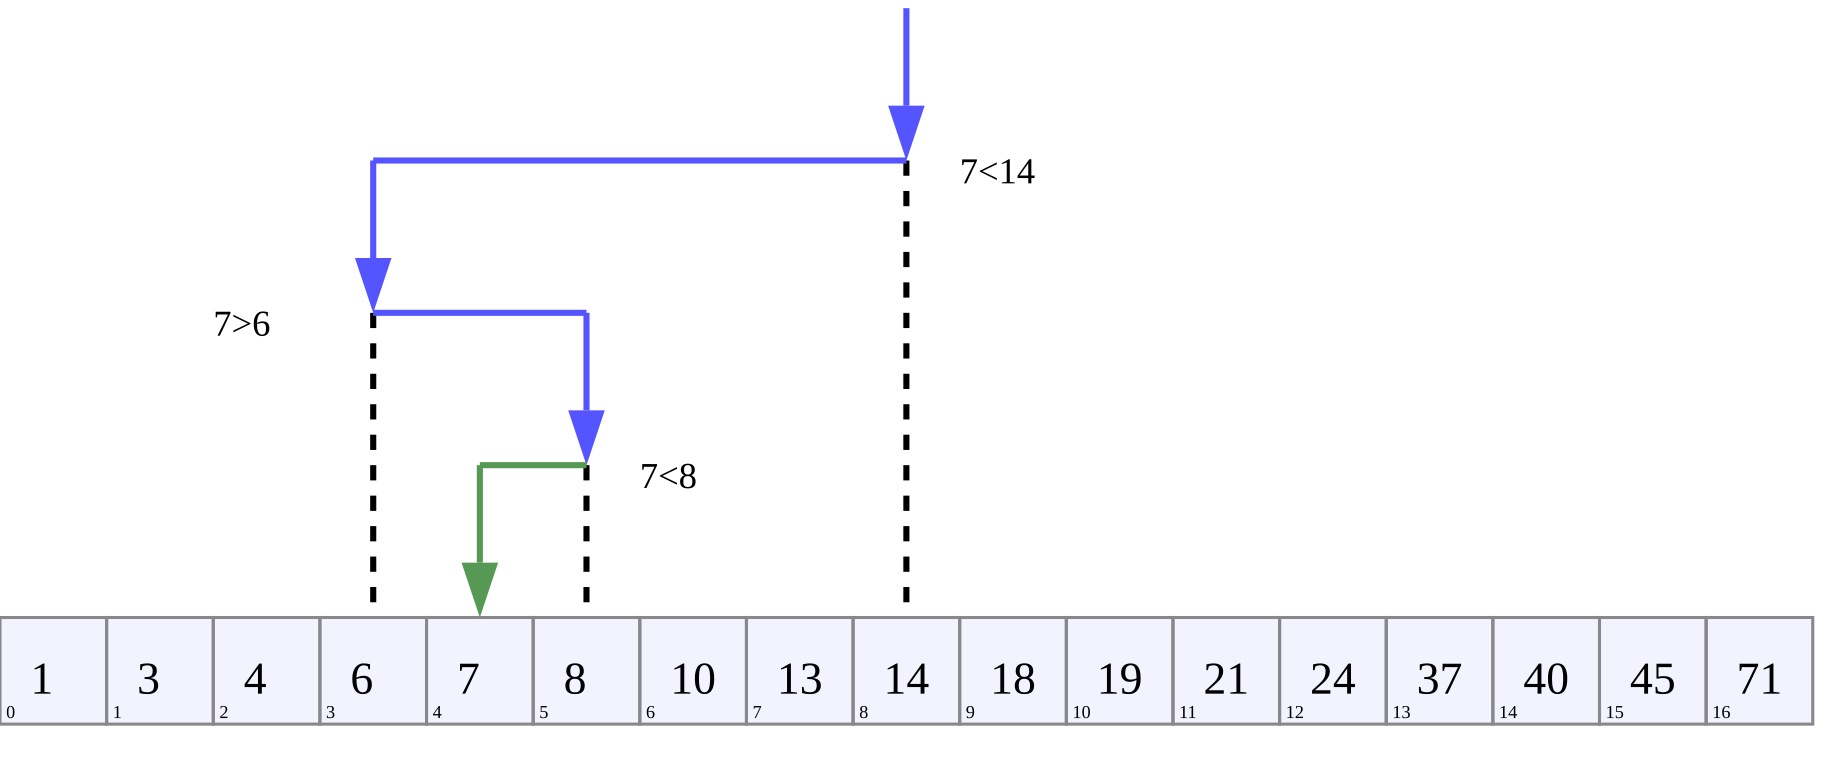
\includegraphics[width=.8\textwidth]{imgs/Binary_Search_Depiction.png}
        \caption{Binary search algorithm, source: \href{https://en.wikipedia.org/wiki/Binary_search}{Wikipedia}\label{fig:binsearch}}
    \end{center}
\end{figure}

Binary search, also known as logarithmic search or binary chop, is a search algorithm that finds the position of a target value within a sorted array: it compares the target to the middle element of the array and, if they are not equal, it eliminates half of the search space by discarding either the left or right half, depending on whether the target value is less than or greater than the middle element. This process is repeated by iteratively searching into the remaining sub-array until the target value is found or the search space is empty. The pseudocode for the algorithm can be seen at \textit{Algorothm} \brref{alg:binsearch}.\\
Binary search runs in logarithmic time in the worst case, doing $O(\log n)$ comparisons, where $n$ is the number of elements in the array, making it much faster than linear search with large arrays thanks to its scaling.\\

\begin{algorithm}
    \captionsetup{labelsep=newline}
    \caption{Pseudocode for binary search algorithm \label{alg:binsearch}}
    \begin{algorithmic}[1]
        \State looking for element $key$
        \State let $L=0$ \Comment{First half}
        \State let $R=n-1$ \Comment{Second half}
        \While{$L\leq R$}
            \State $m=\lfloor (L+R)/2 \rfloor$
            \If{$A[M] < key$}
                \State let $L=m+1$
            \ElsIf{$A[M] > key$}
                \State $R = m - 1$
            \Else
                \State \Return $m$ \Comment{Found}
            \EndIf
        \EndWhile
        \State \Return false \Comment{Not found}
    \end{algorithmic}
\end{algorithm}

\subsection{Exponential Search}

\begin{figure}[H] 
    \begin{center}
        \includegraphics[width=.8\textwidth]{imgs/exponential_search.png}
        \caption{Exponential search algorithm, source: \href{https://www.tutorialspoint.com/data_structures_algorithms/exponential_search.htm}{Tutorialspoint}\label{fig:expsearch}}
    \end{center}
\end{figure}

Exponential search, also called doubling or galloping search, is an algorithm for searching sorted, unbounded lists: there are numerous implementations, most common being determining a sub-array into which the \verb|key| may resides in and performing a binary search \brref{sec:binsearch} within its range.\\
To be more precise: we go trough the list in exponentially increasing steps, with a factor of $2^k$ such that we first look into \verb+list[0]+, then \verb+list[1]+, then \verb+list[2]+, \verb+list[4]+, \verb+list[8]+, following with \textit{16}, \textit{32}, \textit{64}, \textit{128} and so on until we find a value that is greater than the \verb|key|. Once we find it, we perform a binary search between the previous jump and the current (or the end of the array): $2^{k-1} \leq key \leq min(2^{k},n)$.

The algorithm can be more efficient than binary search, as it runs in $O(\log i)$ time, where $i$ is the index of the element being searched for, which could be half if not less than $n$.\\
The pseudocode can be seen at \textit{Algorithm} \brref{alg:expsearch}.\\

\begin{algorithm}
    \captionsetup{labelsep=newline}
    \caption{Pseudocode for exponential search algorithm \label{alg:expsearch}}
    \begin{algorithmic}[1]
        \State looking for element $key$
        \State let $i=0$ 
        \State let $k=0$
        \While{($key>list[i+2^k]$ and $i<n$)} 
            \State $i=i+2^k$ \Comment Gallop to next step
            \State $k=k+1$ \Comment Increment exponent
        \EndWhile
        \If{$i<n$}
            \State binary\_search($list$, $key$, $i$, $min(i+2^k,n)$) 
        \Else
            \State \Return false \Comment{Not found}
        \EndIf
    \end{algorithmic}
\end{algorithm}

\subsection{Extrapolation and Intrapolation \label{sec:extrapol}}

TODO maye or maybe not 

\section{Intersection Algorithms}

\subsection{Brute Force \label{sec:bruteforce}}

The first idea that would come to mind when thinking about intersecting two lists is to simply iterate through both of them and check if the elements are equal: this is the \textit{brute force} approach, which is simple but inefficient. \\
With a time complexity of $O(m \cdot n)$, assuming lists sizes $n$ and $m$ to be around $10^6$, and assuming a modern computer able to do $10^9$ operations per second, this algorithm would need ten minutes to compute a 2-words query, which is less than ideal.\\
The (very short) pseudocode can be seen at \textit{Algorithm} \brref{alg:bruteforce}.\\

\begin{algorithm}
    \captionsetup{labelsep=newline}
    \caption{Pseudocode for brute force algorithm \label{alg:bruteforce}}
    \begin{algorithmic}[1]
        \ForAll{$i=0$ to $n-1$}
            \ForAll{$j=0$ to $m-1$}
                \If{$A[i] == B[j]$}
                    \State add $A[i]$ to result
                \EndIf
            \EndFor
        \EndFor
    \end{algorithmic}
\end{algorithm}

\subsection{Bunny Race}

\begin{figure}[ht] 
    \begin{center}
        \includegraphics[width=.8\textwidth]{imgs/bunny_search.png}
        \caption{Bunny race algorithm \label{fig:bunnyrace}}
    \end{center}
\end{figure}

This approach, often called merge-based, is simple, elegant and fast: the main idea is to have two indices pointing at the two list running after each other by comparing elements each time and incrementing the index pointing at the smallest one (or incrementing both if they are equal).\\ 
To clarify: lets say we have two lists, $A$ and $B$, of size $n$ and $m$ respectively. We start with two pointers, $i$ and $j$, both set to zero. \\
We compare the elements at these indices, $A[i]$ and $B[j]$: if they are equal, we add the element to the result and increment both pointers. \\
If $A[i] < B[j]$, we increment $i$, while if $A[i] > B[j]$, we increment $j$. \\
This process continues until one of the pointers reaches the end of its respective list.\\
The correctness can be proven inductively, exploiting the following observation: if $A[i] < B[j]$ then $A[i]$ is smaller than all elements following $B[j]$ in $B$ since its ordered, so $A[i] \notin B$. The other case is symmetric. \\
In regards to time complexity, we just need to note that at each step the algorithm executes one comparison and advances at least one iterator, thus, given that $n=|A|$ and $m=|B|$, the algorithm runs in no more than $O(n+m)$ time.\\
This time complexity is significantly better than the \textit{brute force} \brref{alg:bruteforce} approach, since it can compute a 2-word query in $10^{-3}$ seconds. \\
The pseudocode can be seen at \textit{Algorithm} \brref{alg:bunnyrace}.

In the case that $n=\Theta (m)$ this algorithm is optimal, because we need to process the smallest set, thus $\Omega(min(n,m))$ is an obvious lower bound. Moreover, this procedure is also optimal in the disk model since it takes $O(\frac{n}{B})$ I/Os. \\
In the case that $n \ll m$ the classic \textit{binary search} can be helpful since we can design an algorithm that search in $A$ for each elements of $B$ in $O(m \log n)$ time, which is better than $O(n+m)$ when $m=o(\frac{n}{\log n})$.

\begin{algorithm}
    \captionsetup{labelsep=newline}
    \caption{Pseudocode for bunny race algorithm \label{alg:bunnyrace}}
    \begin{algorithmic}[1]
        \State let $i=0$ 
        \State let $j=0$ 
        \While{$i<n$ and $j<m$}
            \If{$A[i] < B[j]$}
                \State $i=i+1$ \Comment Increment first
            \ElsIf{$A[i] > B[j]$}
                \State $j=j+1$ \Comment Increment second
            \Else
                \State add $A[i]$ to result \Comment Found
                \State $i=i+1$  \Comment Increment both
                \State $j=j+1$
            \EndIf
        \EndWhile
    \end{algorithmic}
\end{algorithm}